\subsection{Spændingsforsyning}
For at opfylde kravene, der er specificeret i \autoref{sec:krav_spaending}, vælges det at benytte en færdigudviklet komponent, som benytter to $1,5~V$'s AA-batterier, der sidder i en spændingsregulator. Batteriernes kobling danner et split supply. De andre poler, som ikke anvendes til jordforbindelse, benyttes som systemets positive spændingsforsyning, ${V}_{cc}$ og negative spændingsforsyning, ${V}_{dd}$.

Spændingsregulatoren sørger for at give en konstant spænding på henholdsvis $3,4~V$ og $\pm 5,5~V$.\fxnote{Dette gøres ved, at spændingsregulatoren oplagrer spænding fra de to tilkoblede batterier i spoler, når switchfunktionen lukkes. Switchfunktionen åbnes, når spolerne er mættede og en spænding ledes videre i kredsløbet via en diode. Denne switchfunktion åbner og lukker skiftevis i kort tid, hvilket resulterer i, at en konstant spænding ledes til systemet hele tiden.} På sigt vil spændingsforsyningen ikke være i stand til at levere en jævn spænding grundet afladning af batterierne. I dette tilfælde vil spændingsregulatoren indikere dette ved at få en LED til at blinke, når der ikke leveres en konstant spænding. Yderligere vil LED'en stoppe med at lyse, når batterierne er helt afladede. 
Konfigurationen af spændingsforsyningen fremgår af \autoref{fig:spaendingsforsyning}, hvor terminalerne for $\pm 5,5~V$ fremgår som rød(V+) og blå(V-) og grå(Gnd), mens der på den modsatte side fremgår terminalerne for $3,4~V$ som grøn(Vcc) og grå(Gnd). 

\begin{figure}[H]
\centering
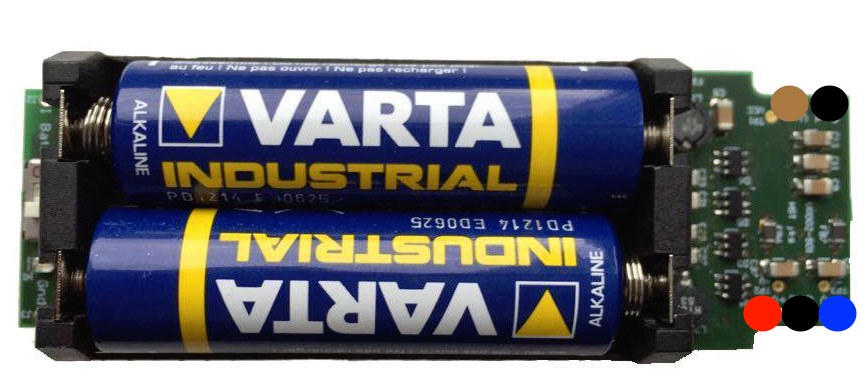
\includegraphics[width=0.6\textwidth]{figures/spaendingsforsyning}
\caption{Spændingsforsyning, der består af to $1,5~V$ batterier i et split supply. Den røde prik illustrerer V+, den blå V-, den grå Gnd og den grøn Vcc.}
\label{fig:spaendingsforsyning}
\end{figure}

